\chapter{関連研究}
\label{chap:previous}
\fancyhf{}
\rhead{\thepage}
\lhead{第\ref{chap:previous}章 関連研究}
\cfoot{\thepage}


本研究が対象とする知識獲得予測の研究は,
学習科学の発達や,
オンライン教育サービスの普及,
教育分野における大規模分析の活発化,
深層学習やその他の多様な分析技術の進展などにより発展してきた研究分野である.
本章では,そのような関連研究を俯瞰し,
現状や周辺概念を整理することで,本研究の学術的位置づけを明確にする.


%まず,教育の個人最適化に関する現状や研究について整理した後,
まず,人間の学習効果について研究する学習科学の歴史と情報技術の発達との関係性について整理した後,
教育と情報技術の象徴的な例であるオンライン教育サービスについて,具体的な事例を挙げながら,その効果や関連する研究について述べる.
次に,深層学習について概説し,本論文との関わりが深いRecurrent Neural Netoworksについて詳細に述べる.
さらに,知識獲得の予測手法であるKnowledge Tracingについて,その有益性や,伝統的な手法,深層学習を用いた最先端の手法について整理した後,
本研究において既存手法を拡張する上で用いる,大規模データから次元削減を行う関連手法について整理する.
最後に,以上の関連研究を踏まえて,
本論文で使用する類似の用語について,定義を明確にする.


\section{学習科学と情報技術}

%学習科学(Learning Sciences)という言葉は,1991年にThe Journal of The Learning Sciencesの国際会議で登場した学問分野である[参考文献引用].
20世紀後半,人間の心の働きを理論化する認知科学が,現実社会で実際に役立つ科学として再構築される流れの中で,
人を日常の学びの中で今より賢くするために実際に役立つ科学として「学習科学(Learning Sciences)」の分野が確立された\cite{白水始2014学習科学の新展開}.
学習科学は,従来の,実験室環境でのみ観測されるような非実用的な理論研究を避け,
学習がうまくいく要因や状況を解明した上で,その学習を人間が積極的に引き起こすことを目指すような,実践の学を新たに打ち立てることを目指したものであった.
明確な定義は様々であるが,\cite{三宅なほみ2002学習環境のデザイン実験}らは
「よりよい教育を実現したいという社会的要請を背景にして,これまでの認知研究に基づき,
現実の人の学習,例えば学校教育の中での子どもたちの学習を研究し,
現代のテクノロジを駆使して実効性のある教育のシステムを教育実践の中で作り上げようという研究動向」
と定義している.


学習科学の発展は,
認知科学の進展だけでなく,情報技術の発達が大きな貢献を果たしている.
学習科学は,人間の認知過程を解明する基礎研究としての性質に加え,
実社会での有効性を検証する実証的な応用研究としての性質を兼ね備えているため,
オンライン教育サービスのような教育と情報技術の融合によって,
これまで実現しにくかった学習環境を作り検証できるようになったことは,
学習科学の発展を大きく加速させた.

そうした情報技術との融合により実証研究が進み,今日注目されている教育システムの例としてアダプティブラーニングが挙げられる\cite{carbonell1970ai, midgley2014goals}.
アダプティブラーニングは,個人に最適化された学習内容の自動提供を実現するもので,
その社会的影響の大きさからアメリカを中心として世界的に注目が集まっており,関連するスタートアップや大学での研究に多額の資金が投入されている\cite{piccioli2014learning}.

学習内容を個人に最適化させるという考え自体は,
学習科学の研究においても,また,研究という形に上がらないレベルでも,古くから存在し,
例えば習熟の遅い生徒に教師が個別で補習に当たったり,
個別指導塾や通信教育で生徒各自が自身の習熟度に見合った講義を受けたりと,
様々な形態を取って実践されてきた.
しかし,こうした従来の方法は,
教育の粒度を細かくし,個人最適化を図ろうとするほど,
教師一人あたりが担当できる生徒の数が減ることによる人材的・金銭的負担や,
教師ごとの指導能力の違いなどの問題に直面し,
すべての生徒に最適な学習内容を提供するという目的を達成するには障壁が残っていた.

この事態を打開したのが,教育と情報技術の融合である.
中でも,その象徴ともいえるオンライン教育サービスでは,
サービスを利用する生徒の学習行動ログを収集することで,
これまで困難であった大規模な学習効果分析を可能にしたことに加え,
オンライン上の学習コンテンツを生徒が個人で利用するという形態を活かし,
研究成果を元に学習コンテンツを個人に最適化して提供することを容易にした.


このように,基礎理論に加え実証性も重視する学習科学の領域は,
情報技術との融合により大きく発達してきた.
特に,オンライン教育サービスは,
データの蓄積と研究,そして研究成果の実証という3つの目的が達成できるプラットフォームとして,
大きな注目を集めている.



\section{オンライン教育サービスと大規模な学習効果分析}
オンライン教育サービスの代表的な例としてMassive Open Online Courses(MOOCs)とIntelligent Tutoring System(ITS)を取り上げ,
具体的な事例を挙げながら,関連する研究について述べる.
また,こうしたオンライン教育サービスが大規模分析に活用されている状況や研究について整理する.


\subsection{MOOCsとITS}
MOOCsはMassive Open Online Courses\cite{mcauley2010mooc, pappano2012year,siemens2013massive}の略称で,
特に日本語で表記する場合は大規模公開オンライン講座と記述することがある.
MOOCsは,オンライン上で公開された,大学などの様々な教育機関の講座を,誰もが無償で受講でき,また修了時には修了証も取得できる教育サービスのことを指す.

学びたい人がいつでもどこでも学習リソースにアクセスできる,というMOOCsの概念自体は古くから提唱されていたが,
実現化したのは,2008年にカナダのマニトバ大学で学生向けのオンライン講座を開設した際に,
25人の受講者だけでなく2000人以上の人がその講座に参加したことがきっかけだと言われている\cite{yuan2013moocs}.

以前から,大学などの高等教育機関は,
オープンコースウェア\cite{abelson2008creation}という形で講義の動画や資料を公開していたが,
MOOCsは,参加人数が非常に大規模で,また,高等教育水準の内容だけでなく,初等中等教育水準の内容の講座も含まれている点で異なる.
また,これまでもオンラインの講座というものは存在していたが,
MOOCsは,
参加人数が非常に大規模である点や
公開している講座の数が大規模である点,
また,その内容が多様であるという点,
利用が無料,あるいは無料に近いという点において,
これまでのオンライン講座とは異なる.


MOOCsは,従来の,学校の教室で一斉授業形式で提供される教育形態と異なり,
オンライン上の多様な講座に生徒が個人でアクセスし,
講座ごとに提供される講義の動画や演習システムなどを通じて,
いつでもどこでも,自身の習熟度合いやペースに合わせて,学習したいものを選択して学習できる.
従来の教育の,生徒が自身の習熟度合いに見合った学習ができないという問題を解決するものとして注目されていることに加え,
産業や社会への影響も注目されている.
例えば,大学生や社会人でも,自身の専門領域に関する講座を受講することでより理解を深めたり,
あるいは専門領域とは異なる幅広い講座を受講することで教養を養ったり,
自身に必要な資格に関する講座を受講することで,キャリアを設計したりできる.
また,公教育の整備が追いついていないような発展途上国においては,
MOOCsが教育に与える影響は大きく,その影響や可能性を分析する報告は多い\cite{trucano2013more,liyanagunawardena2013impact}.

このように,MOOCsは社会の多様な場面で,これまでにない学習機会を提供しており,
教育や学習といったもののあり方に大きな影響を与えている.


\begin{figure}[t]
\begin{center}
%\hspace*{-40pt}\makebox[1.2\textwidth][c]{
%\makebox[1.2\textwidth][c]{
\hspace*{-20pt}
\makebox[1.1\textwidth][c]{
	%\begin{center}
	\minipage{0.55\textwidth}
		\centering
\includegraphics[width=200pt]{./img/coursera.pdf}
		\caption{Coursera}
		\label{fig:cousera}
	\endminipage
	\hfill
	%\end{center}	
	%\begin{center}
	\minipage{0.55\textwidth}
		\centering
\includegraphics[width=200pt]{./img/jmooc.pdf}
		\caption{JMOOC}
		\label{fig:jmooc}
	\endminipage
	%\end{center}	
}
\end{center}
\end{figure}

MOOCsの有名な事例として,世界的に有名なCoursera(図\ref{fig:cousera})や,日本発のMOOCsであるJMOOC(図\ref{fig:jmooc})が挙げられる.
Courseraは,2017年1月の時点で,
29の国にまたがる148の教育機関とパートナーシップを結び,
コンピュータサイエンス,数学や論理,社会科学などに関する1600以上の講座を,2200万人以上に提供している\footnote{講座数と利用者数はトップページの記載より引用.}.
JMOOCは,2013年11月に日本版のMOOCsとして設立され,
10代から80代までと幅広い年代に,アートや医療,自然科学や資格試験対策などの講座を提供しており,
2017年1月の時点で,140の講座を50万人以上が受講している\footnote{講座数と利用者数はトップページの記載より引用.}.


多様な講座を多くの人に提供するMOOCs以外にも,
より個人の学習過程をサポートすることを目的として設計された,
Intelligent Tutoring System(ITS)と呼ばれるオンライン自動学習支援システムの利用も拡大している\cite{sleeman1982intelligent}.

\begin{figure}[htb]
\begin{center}

\includegraphics[width=200pt]{./img/knewton.pdf}
\end{center}
\caption{Knewtonのイメージ}
\label{fig:knewton}
\end{figure}

ITSの有名な事例として,世界最大級のITSであるKnewton\footnote{\url{https://www.knewton.com/}}(図\ref{fig:knewton})が挙げられる.
Knewtonでは,生徒の学力や理解度と,学ぶべき対象をマッピングすることで、
生徒個人に最適な学習過程を設計し,
かつ生徒の学習の進捗に応じてその過程を動的に変化させる仕組みを有している\cite{upbin2012knewton}.


また,近年では,これまで難しいと言われていたITSのMOOCsへの埋め込みを達成したとする研究\cite{aleven2015beginning}も報告されており,
ITSが利用される場面は,今後より拡大していくといえる.



\subsection{学習行動ログの蓄積と大規模分析の活発化}

MOOCsやITSなどのオンライン教育サービスには,
人々に新たな学習の機会を提供するという側面だけでなく,
これまで困難であった大規模な学習効果分析の可能性を高めるという側面もある.

生徒はオンライン上で提供された講義動画や演習問題を通して学習するが,
オンライン上で実施されているため,学習行動ログをデータとして蓄積することができ,蓄積されたデータを分析に活用することができる.
多様な生徒が利用するため,多様な生徒の大規模な学習行動ログから多様な講座の学習効果の分析が可能となりつつある.

特に,演習問題の回答ログはその演習問題により評価される知識を生徒が獲得しているか否かを表現しているため,知識獲得の分析に利用できる.
例えば,MOOCsの演習問題の回答ログを利用して知識獲得の予測を行う研究\cite{machardy2015toward}では,
世界的に有名なMOOCsであるKhan Academyから収集したデータを利用していたが,
その問題回答ログ数は100万件以上であり,
これまでにないほど大規模なデータを対象に分析が実施されたといえる.


\subsection{実証性の高いプラットフォームとしての性質}

さらに,オンライン教育サービスが学習効果分析の価値を大きく高めている要因として,
オンライン上のコンテンツを,多様な生徒が,個人で利用するというプラットフォームとしての性質がある.

現在の学校教育の形態では,生徒の学習効果に関する分析を行い,なんらかの知見を得たとしても,
それを多様な生徒に適用して効果を検証したり,各個人に提供できるような環境が整備されておらず,
学習効果分析が社会に与える影響が限定的であった.
また,従来の一般的なeラーニングによる学習支援システムも,
大学のような各教育機関が個別に設定し,学内の生徒が利用者の中心であったため,
システムの利用者が限定されており,データの多様性や研究成果の活用可能性も狭い範囲に留まっていた.


一方,MOOCsやITSのような大規模なオンライン教育サービスは,
教育機関の垣根にとらわれず,多様な背景,適性,能力を持つ生徒が利用していることに加え,
学習コンテンツを個人が利用する形態のため,
多様なデータを元に得られた一般性のある知見を,多様な生徒に対して,生徒個人の粒度で提供することが可能である.
例えば,生徒の知識獲得予測の研究は,得られた成果から,
より生徒の学習効率を高めたり,継続を推進するような教材推薦システムを開発し,
実際のサービス上で個人個人に適用することで,効果を実証することができる.
このような性質から,オンライン教育サービスのデータに基づいた学習効果分析が持つ
社会的影響は,大きなものとなっている.
%そのため,知識獲得の予測を始めとする,学習効果分析によって得られた成果に基づいた,
%学習の効率化や継続を促進する教材推薦システムの開発が持つ社会的影響が大きなものとなっている.




\section{深層学習}

本研究で用いる技術の核となっている,深層学習について述べる.
まず,深層学習の基礎となっているニューラルネットワークの概念について説明した後,
深層学習の概要について述べ,
さらに本研究で用いる深層学習モデルであるRecurrent Neural Networksについて詳述する.



\subsection{ニューラルネットワーク}
深層学習は,機械学習における一分野であり,
その中でもニューラルネットワークという特殊なモデル構造を拡張したものである.
よって,まずはニューラルネットワークについて説明する.

ニューラルネットワークは,機械学習におけるモデル構造の一つで,人間の脳の神経回路の仕組みを模したものである.
人間の脳は,膨大な数のニューロンと呼ばれる神経細胞から構成され,
各ニューロンは相互に連結し,巨大なネットワークを成している.
外界からの情報によってあるニューロンが刺激を受けると,そのニューロンの電位は次第に上昇し,
電位が一定の閾値を超えるとそのニューロンは発火,接続している他のニューロンに情報の信号を出力することにより,情報の伝達が行われている.
ニューラルネットワークのモデルでは,
このニューロン一つ一つの情報伝達の仕組みと,
それらが互いに接続してネットワークを成す構造をモデル化している.

各ニューロンは図\ref{fig:neuron}のようにモデル化される.

\begin{figure}[htb]
\begin{center}
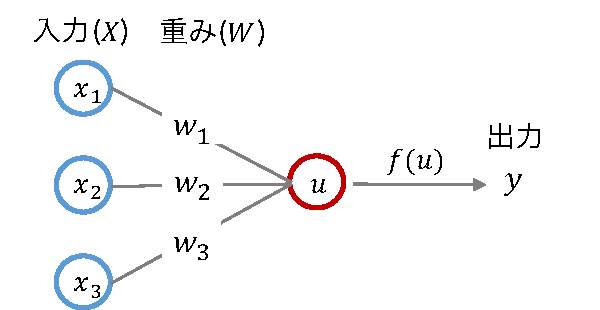
\includegraphics[width=200pt]{./img/neuron.pdf}
\end{center}
\caption{各ニューロンの仕組み}
\label{fig:neuron}
\end{figure}

各ニューロンは他のニューロンから入力信号$x_i$を受け取るが,その信号の伝達効率は一様ではない.
それぞれの入力には伝達効率として重み$w_i$が設定され,その重み付きの入力$w_i x_i$が対象のニューロンに加算されていく.
%その総和$u$がある閾値$\theta$を超えた時,該当のニューロンは発火したものと見なし,他のニューロンに出力信号$y$が送られる.
その総和$u$は事前に定められた活性化関数$f$に基づいて正規化され,出力される.
活性化関数には様々な種類があり,
式\ref{eq:step}で表されるような,閾値$\theta$を境に0か1を出力するような単純なステップ関数以外に,
式\ref{eq:sigmoid}, \ref{eq:tanh}で表されるようなシグモイド関数(sigmoid),双曲線正接関数(tanh)などの非線形関数も存在する.

\begin{eqnarray}
\label{eq:step}
%\varphi(x) = f(x - \theta) = \left\{
f(x) = \left\{
	\begin{array}{l}
	1 \text{ if } x \geq \theta \\
	0 \text{ if } x < \theta
	\end{array}
\right.
\end{eqnarray}

\begin{eqnarray}
\label{eq:sigmoid}
%\varphi(x) = \frac{1}{1 + e^{-x}}
f(x) = \frac{1}{1 + e^{-x}}
\end{eqnarray}

\begin{eqnarray}
\label{eq:tanh}
%\varphi(x) = \frac{e^x - e^{-x}}{e^x + e^{-x}}
f(x) = \frac{e^x - e^{-x}}{e^x + e^{-x}}
\end{eqnarray}



\begin{figure}[t]
\begin{center}
%\hspace*{-40pt}\makebox[1.2\textwidth][c]{
\hspace*{-40pt}\makebox[1.1\textwidth][c]{
	\minipage{0.55\textwidth}
		\centering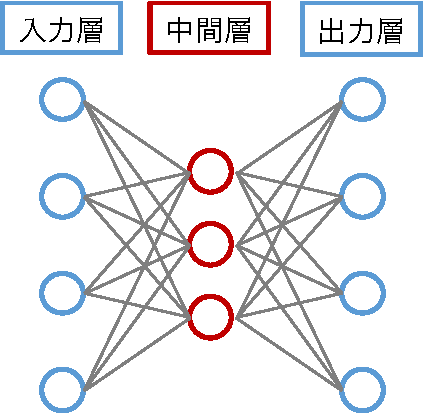
\includegraphics[height=150pt]{./img/neuralnetwork.pdf}
		\caption{単純パーセプトロンの構造}
		\label{fig:neuralnetwork}
	\endminipage\hfill
	\minipage{0.55\textwidth}
		\centering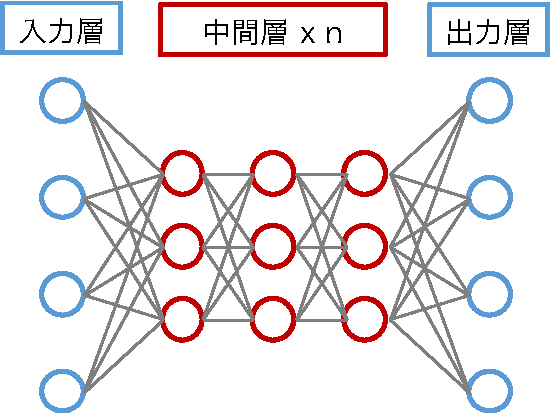
\includegraphics[height=150pt]{./img/deeplearning.pdf}
		\caption{多層パーセプトロンの構造}
		\label{fig:deeplearning}
	\endminipage\hfill
}
\end{center}
\end{figure}


このようにモデル化された各ニューロンを,人間の脳の神経回路のように,互いに結合させてネットワーク化した例が図\ref{fig:neuralnetwork}である.
これは1958年にRosenblattにより提案された単純パーセプトロンというネットワークで,
二ューラルネットワークの元祖とも言われる最も基本的なネットワークである\cite{rosenblatt1958perceptron}.
それぞれのニューロン(以下,ユニット)は,各層の間で互いに全結合しており,
前の層からの入力${\bf x}$に重み${\bf W}$が掛け合わされ,バイアス項${\bf b}$を加算したものに活性化関数$f$が適用され,出力される.
層$i$から層$j$への出力の計算は以下の式に基づいて行われる.
\begin{eqnarray}
{\bf y}_j =  f({\bf W}_{i,j} {\bf x}_i + {\bf b}_j)
\end{eqnarray}
なお.
${\bf x}_i$は層$i$における出力($i=1$の時はモデルへの入力)を指し,
${\bf W}_{i,j}$は重み行列を指し,
${\bf b}_j$はバイアス項を指し,
$f$は活性化関数を指し,
${\bf y}_j$は層$j$における出力を指す.

この計算を層ごとに順次行い,最終的な出力が決定され,事前に設定した誤差関数によってモデルの予測誤差が算出される.
誤差関数は平均二乗誤差や交差エントロピー誤差など,目的に応じて様々であるが,
ニューラルネットワークでは,この誤差関数を重みやバイアスのパラメータによって微分して負の勾配方向を見つけ,
パラメータを勾配方向に修正することを繰り返すことにより,最適なパラメータを探索していく.
重みの更新の基本的な仕組みは,以下の式によって表される.
\begin{eqnarray}
\nabla E &=& \frac{\partial E}{\partial {\bf W}_{i,j}}
\\
{\bf W}^{(t+1)}_{i,j} &=& {\bf W}^{(t)}_{i,j} - \epsilon \nabla E
\end{eqnarray}
なお,
$E$は誤差関数であり,
${\bf W}^{(t)}_{i,j}$は時刻$t$における重み行列であり,
$\epsilon$は学習率と呼ばれる,1回の学習あたりのパラメータ更新量の大きさを決定する定数である.

このようにニューラルネットワークの基礎として考案された単純パーセプトロンだが,
排他的論理和(XOR)のような非線形問題を解けず,現実の複雑な問題には適用できないことが指摘された\cite{minsky1969perceptron}.
また,ニューラルネットワークを多層にすることも早くから考案されていたが,
極めて高い計算処理性能を要することが課題であり,長い間実用には堪えない時代が続いていた.
このような歴史を経た後,近年の計算機の性能向上や,その他のモデル設計上の技術的進歩を背景に,
ニューラルネットワークをさらに多層に重ねて,より複雑な特徴を抽出し,非線形問題も含めた様々な問題を扱えるように設計されたのが深層学習である.


\subsection{深層学習の概要}
深層学習は,機械学習における一分野で,ニューラルネットワークを多層に重ねたものである.
画像処理に利用されるConvolutional Neural Networks\cite{lecun1998gradient}や
系列データの処理に利用されるRecurreut Neural Networks\cite{williams1989learning}など,
目的に応じた様々な拡張があるが,どれも図\ref{fig:deeplearning}のような多層パーセプトロンというモデル構造を基本としている.
多層パーセプトロンも,層間の信号の伝搬など,基本的な構造は単純パーセプトロンと大きな違いはない.
しかし,隠れ層が多層になったことで,パラメータ更新の際に何層にも渡って微分の連鎖規則を繰り返すことが必要になり,計算コストが膨大になってしまう.
そのため考案されたのが誤差逆伝搬法\cite{rumelhart1988learning}である.
誤差逆伝搬法では,出力結果に基づいて,
出力層から入力層に向かって順番に重みを修正する手法により,
複雑な問題を説明するようなユニット間の重みを学習できるようになり,
非線形問題も解くことが可能になった.

この誤差逆伝搬法や,確率的勾配降下法\cite{robbins1951stochastic,kushner2003stochastic},AdaDelta\cite{zeiler2012adadelta},Adam\cite{kingma2014adam},Nadam\cite{dozat2015incorporating}などのより効率的な勾配降下法,モデルの過学習を抑制するdropout\cite{srivastava2014dropout}と呼ばれる機構など,
様々な技術的工夫が考案されたことにより,
現実的な計算コストで効率的に深層学習を行うことが可能になり,深層学習を用いた研究活動が急速に活発化した.


深層学習の活用により,
画像認識\cite{schroff2015facenet,szegedy2014going},
音声認識\cite{hinton2012deep, bahdanau2015end},
会話認識\cite{sak2015fast},
機械翻訳\cite{sutskever2014sequence, dong2015multi},
質問応答文生成\cite{yin2015neural},
画像説明文生成\cite{xu2015show,vinyals2014show}等,
多様な研究領域で飛躍的な進展が報告がされている.
特に,直近の一年間だけでも
画像から動画を生成する研究\cite{vondrick2016generating}や,
会話を人間と同程度に認識できるとする音声認識の研究\cite{xiong2016achieving},
一部の欧米言語間の文レベルで,ほぼ人間と同等に正確な翻訳を実現したとする機械翻訳の研究\cite{wu2016google}などを始めとする数々の報告がされており,
深層学習によって,日々驚異的な成果が生み出されている.

また,2016年3月に人間のプロを倒したことで一躍有名になった,Google Deep Mindが開発したコンピュータ囲碁プログラムの「AlphaGo」\cite{silver2016mastering}は,
過去の人間が打った大量の棋譜に深層学習を適用した後,自己対局による強化学習を通して,
今後10年は不可能と言われていた,人間のプロを打ち負かすほどの棋力を獲得した.
AlphaGoは,過去の対局の情報である棋譜の分析によって人間を真似ただけでなく,
それまで人間が考えつかなかったような手を学習しており,囲碁界に衝撃を与えている.
このように,深層学習は,人間が認識できないようなデータの複雑な特徴を捉えることで,
これまで人間が作り上げてきた概念を大きく塗り替える可能性を秘めている.


%大規模データが必要であることに言及
一般に,深層学習モデルを学習させる際には,大規模な訓練データが必要となる.
深層学習モデルが,人の手で素性を設計していない生の訓練データから,特徴的な表現を学習し,最適化するには,
膨大な数の内部パラメータを設定して学習することが必要となる.
ときには数十万から数百万以上の内部パラメータが設定されることもあり,
こうした膨大な数のパラメータを学習するには,大規模な訓練データが必要となる.
データ数が不足すると,データの潜在的な特徴を十分に学習できないことに加え,
汎用性の低い特徴まで過剰に学習してしまう過学習に陥りやすくなる\cite{tetko1995neural}.

実際に大規模データを利用した研究の例では,
人間より高い精度で人の顔を見分けられると報告する顔認識の研究\cite{schroff2015facenet}では数百万人の2億枚以上の顔画像を,
英語からフランス語に翻訳する機械翻訳の研究\cite{xu2015show}では1200万もの文章を,
それぞれ訓練データとして利用している.



\subsection{Recurreut Neural Networks}
深層学習のネットワークには,目的に応じたいくつかの種類があるが,
ここでは,知識獲得の予測に深層学習を適用した手法\cite{piech2015deep}に用いられていた,Recurreut Neural Networks\cite{williams1989learning}(以下,RNN)について説明する.


RNNは深層ニューラルネットワークの一種で,主に系列データの解析に利用される.
系列データとは,同質のデータを直列に並べて表現することにより,特定の意味を持ったデータのことで,
例えば,時系列に沿って変化する株価のようなデータや,順序性を持って並ぶ単語から構成される文章などのデータが系列データにあたる.

近年,RNNはデータの大規模化や計算機性能の向上などにより,幅広い領域の系列データに対して適用されるようになった.
具体的には,
機械翻訳\cite{sutskever2014sequence, dong2015multi},
手書き文字認識\cite{graves2009offline,louradour2014curriculum},
音声認識\cite{hinton2012deep,bahdanau2015end},
ユーザログ解析\cite{hidasi2015session},
画像説明文生成\cite{xu2015show,vinyals2014show},
医療診断\cite{choi2015doctor,lipton2015learning}等の領域で高い性能を発揮することが報告されている.

% - RNNの構造の概略
伝統的なRNNは,
入力層,隠れ層,出力層の3層から構成されている.
系列方向を時刻とすれば,
時刻$t$の入力${\bf x}_t$と時刻$t-1$の隠れ層${\bf h}_{t-1}$の情報を入力として,
時刻$t$の隠れ層${\bf h}_t$が式\ref{fig:rnn}のように計算される,
一つ前の情報を繰り返し(recurrent)入力するという構造である.
\begin{eqnarray}
\label{fig:rnn}
{\bf h}_t = f({\bf x}_t, {\bf h}_{t-1})
\end{eqnarray}
なお,関数$f$は活性化関数であり,シグモイド関数や双曲線正接関数,Relu\cite{nair2010rectified},ELUs\cite{clevert2015fast}などの非線形関数が用いられるのが一般的である.
モデル構造は図\ref{fig:rnnFold}のように表され,隠れ層の部分を時間方向に展開して図\ref{fig:rnnUnfold}のように表されることもある.

\begin{figure}[htb]
\begin{center}
\hspace*{-40pt}\makebox[1.1\textwidth][c]{
	\minipage{0.35\textwidth}
		\centering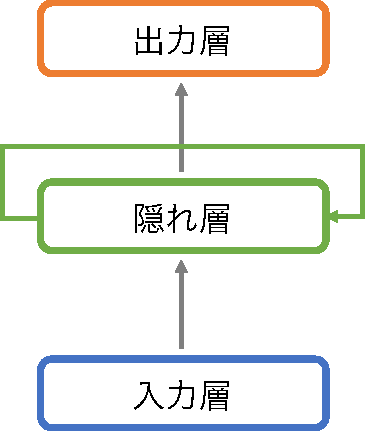
\includegraphics[height=100pt]{./img/rnnFold.pdf}
		\caption{RNNの基本構造}
		\label{fig:rnnFold}
	\endminipage\hfill
	\minipage{0.75\textwidth}
		\centering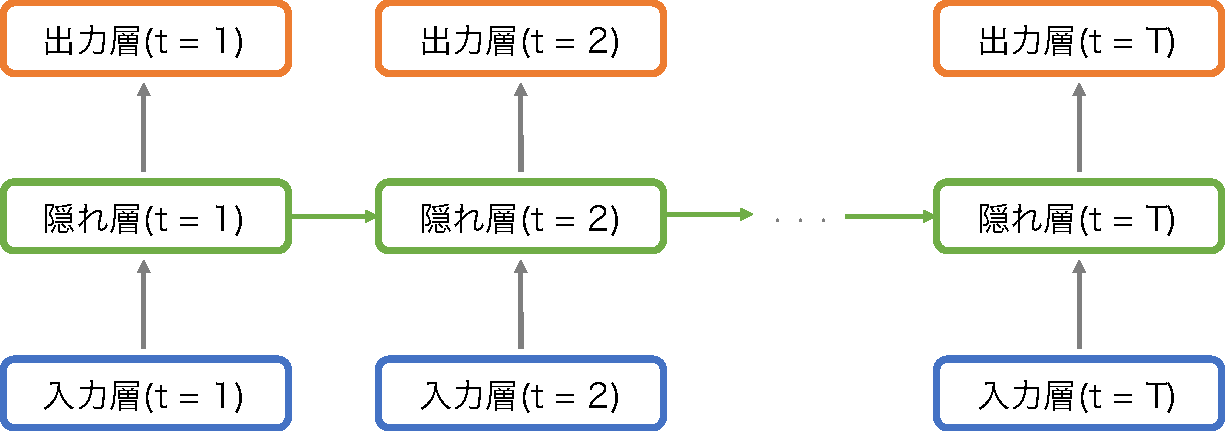
\includegraphics[height=100pt]{./img/rnnUnfold.pdf}
		\caption{RNNの基本構造(展開)}
		\label{fig:rnnUnfold}
	\endminipage\hfill
}
\end{center}
\end{figure}

%関数$f$は,入力である${\bf x}_t$や${\bf h}_{t-1}$をアフィン変換\footnote{平行移動と線形変換を組み合わせた変換のこと.}して足しあわせた後,活性化関数にかけるというものがよく利用される.
%活性化関数はシグモイド関数やtanh(Hyperbolic Tangent関数),Relu\cite{nair2010rectified},ELUs\cite{clevert2015fast}など多く提案されており,通常,非線形関数である.



% - RNNの課題について説明
このように,データの系列に沿った情報を反映して学習できるRNNだが,
長期的な表現になるほど学習が難しくなるという課題がある\cite{bengio1994learning}.
RNNの学習では,様々な勾配法に基づいた最適化が行えるが,どの勾配法を用いる場合においても
式\ref{fig:rnn}に表れるように同じ変換を繰り返し行うため,隠れ層が多層になり,
勾配が爆発して学習モデルが壊れてしまうという勾配爆発\cite{bengio1994learning,pascanu2013difficulty}という問題や,
勾配が消滅して対象データの長期的な特徴量を捉えることができないという勾配消滅\cite{pascanu2013difficulty, hochreiter1998vanishing}という問題が発生する.

% - 課題解決の手法について説明
こうした問題を解決もしくは緩和する手段の一つが,学習時の勾配に制約を加える方法である.
具体的には,
学習させるパラメータの勾配の絶対値の最大値を予め決めておき,
最大値以上の場合にはその最大値になるように勾配の値を置き換える方法\cite{mikolov2012statistical}や,
学習させるパラメータの勾配のノルム\footnote{ベクトルの「長さ」の概念を一般化したもの}の最大値を予め決めておき,
最大値以上の場合にはノルムがその最大値以下になるようにノルムを抑制する方法\cite{pascanu2013difficulty}などが報告されている.


もう一つの手段が,ゲート付き活性化関数の利用である.
先に言及したが,RNNには異なる活性化関数を利用するという形でいくつかの種類がある.
うまく設計された活性化関数を利用することで,勾配消滅を緩和してデータの長期的な特徴をよく捉えられたり,計算コストを削減することができたりする.
以降では,よく研究報告で取り上げられるSimple RNN(以下,SRNN)\cite{williams1989learning},Long Short  Term Momory RNN(以下,LSTM-RNN)\cite{hochreiter1997long},Gated Recurrent Neural Networks(以下,GRNN)\cite{cho2014learning}の3つについて詳細に説明する.



\subsubsection{SRNN}
SRNNはゲート付き活性化関数を用いない単純な構造のRNNである.
\cite{le2015simple, krueger2015regularizing}で報告される工夫を取り入れることで,データの長期的な特徴を効果的に捉えることができるようになるが,
多くの場合で,LSTM-RNNやGRNNのようにゲート付き活性化関数を用いるRNNの方がモデルの性能という点で優れている.

SRNNによる最も単純なモデルの定式は以下の式で定義される.
\begin{eqnarray}
\label{eq:srnn1}
{\bf h}_t &=& \tanh({\bf W}_{xh} {\bf x}_t + {\bf W}_{hh}  {\bf h}_{t-1} + {\bf b}_h)\\
\label{eq:srnn2}
{\bf y}_t &=& \sigma( {\bf W}_{hy} {\bf h}_t + {\bf b}_y)
\end{eqnarray}
ここでは,
$t$は時刻を指し,
${\bf x}_t$は時刻$t$の入力ベクトルを指し,
${\bf h}_t$は時刻$t$の隠れ層を指し,
${\bf y}_t$は時刻$t$の入力ベクトルを元にした予測値を指し,
${\bf W}_{xh}$,${\bf W}_{hh}$はそれぞれ重み行列を指し,
${\bf b}_h$,${\bf b}_y$はそれぞれバイアス項を指し,
$\tanh$は$( e^x - e^{-x} )/( e^x + e^{-x} )$で定義される双曲線正接関数を指し,
$\sigma$は$1 / (1 + e^{-x})$で定義されるシグモイド関数を指す.
訓練時には,重み行列${\bf W}_{xh}$,${\bf W}_{hh}$,${\bf W}_{hy}$とバイアス項${\bf b}_h$,${\bf b}_y$を学習する.


\subsubsection{LSTM-RNN}
LSTM-RNNはLong Short Term Memoryというゲート付き活性化関数を用いるRNNで,
その名前の通り,SRNNでは捉えることが難しかったデータの長期的表現と短期的表現の両方の獲得を目的に開発されたものである\cite{hochreiter1997long}.
LSTM-RNNはSRNNと比較すると,モデルの性能という点で優れているが,内部パラメータの数が非常に大きく,学習コストは大きい.
%最先端の成果を報告する研究でしばしば利用されているが,
%LSTM-RNN自体が開発されたのは1997年でありLSTN-RNNが新しいというわけではない.

LSTM-RNNによるモデルの定式にはいくつか種類が存在するが,特に,後述するDeep Knowledge Tracing\cite{piech2015deep}で用いられるLSTM-RNNは下記の式で定義される.
\begin{eqnarray}
\label{eq:lstmrnn1}
{\bf i}_t &=& \sigma({\bf W}_{xi}{\bf x}_t + {\bf W}_{hi}{\bf h}_{t-1} + {\bf b}_i) \\
\label{eq:lstmrnn2}
{\bf g}_t &=& \sigma({\bf W}_{xg}{\bf x}_t + {\bf W}_{hg}{\bf h}_{t-1} + {\bf b}_g) \\
\label{eq:lstmrnn3}
{\bf f}_t &=& \sigma({\bf W}_{xf}{\bf x}_t + {\bf W}_{hf}{\bf h}_{t-1} + {\bf b}_f) \\
\label{eq:lstmrnn4}
{\bf o}_t &=& \sigma({\bf W}_{xo}{\bf x}_t + {\bf W}_{ho}{\bf h}_{t-1} + {\bf b}_o) \\
\label{eq:lstmrnn5}
{\bf m}_t &=& {\bf f}_t \odot {\bf m}_{t-1} + {\bf i}_t \odot {\bf g}_t \\
\label{eq:lstmrnn6}
{\bf h}_t &=& {\bf o}_t \odot {\bf m}_t  \\
\label{eq:lstmrnn7}
{\bf y}_t &=& \sigma({\bf W}_{my} {\bf m}_t + {\bf b}_y) 
\end{eqnarray}
ここでは,
${\bf i}_t$はInput Gateを指し,
${\bf f}_t$はForget Gateを指し,
${\bf g}_t$はメモリセルへの入力を指し,
${\bf o}_t$はOutput Gateを指し,
${\bf m}_t$はメモリセルを指し,
${\bf W}_{xi}$,${\bf W}_{hi}$,
${\bf W}_{xg}$,${\bf W}_{hg}$,
${\bf W}_{xf}$,${\bf W}_{hf}$,
${\bf W}_{xo}$,${\bf W}_{ho}$,
${\bf W}_{my}$
はそれぞれ重み行列を指し,
${\bf b}_i$,${\bf b}_g$,${\bf b}_f$,${\bf b}_o$,${\bf b}_y$はそれぞれバイアス項を指し,
$\odot$は要素積を指す.

式\ref{eq:lstmrnn5}にあるように,メモリセルへの入力は1つ前のメモリセルの状態${\bf m}_{t-1}$と入力${\bf g}_t$であり,
それぞれの入力に対して,過去のメモリセルからの情報を捨てるForget Gateと現在からの情報を調整するInput Gateを作用させ,${\bf m}_t$を得る.
新しい隠れ層${\bf h}_t$は式\ref{eq:lstmrnn6}のようにメモリセルからの出力をOutput Gateで調整したものを入力として受け取る.
これらのゲートにより,
長期的な特徴と短期的な特徴が捉えられるとされている.

\subsubsection{GRNN}
GRNNはGated Recurrent Unit\cite{cho2014learning}というゲート付き活性化関数を用いるRNNのことで,
GRUはLSTMのように長期的な表現と短期的な表現を捉えるために提案された活性化関数である.
\cite{cho2014learning}らが2014年に発表して以来,GRNN自体やGRNNの活用に関する研究が多く報告されている\cite{chung2014empirical, zaremba2015empirical, chung2015gated, karpathy2015visualizing, biswassentiment, pezeshki2015sequence}.
LSTMよりもパラメータの数が少なく学習コストが小さい傾向にあるが,
LSTM-RNN,GRNNの性能を比較した研究\cite{chung2014empirical, zaremba2015empirical}において両者が同程度の性能であることが報告されている.

GRNNは下記の式により定義される.
\begin{eqnarray}
\label{eq:grurnn1}
{\bf r}_t &=& \sigma({\bf W}_{xr}{\bf x}_t + {\bf W}_{hr}{\bf h}_{t-1} + {\bf b}_r)\\
\label{eq:grurnn2}
{\bf z}_t &=& \sigma({\bf W}_{xz}{\bf x}_t + {\bf W}_{hz}{\bf h}_{t-1} + {\bf b}_z)\\
\label{eq:grurnn3}
\tilde{{\bf h}}_t &=& \tanh({\bf W}_{xh}{\bf x}_t + {\bf W}_{hh}({\bf r}_t \odot {\bf h}_{t-1} + {\bf b}_h))\\
\label{eq:grurnn4}
{\bf h}_t &=& (1 - {\bf z}_t) \odot {\bf h}_{t-1} + {\bf z}_t \odot \tilde{{\bf h}}_t\\
\label{eq:grurnn5}
{\bf y}_t &=& \sigma( {\bf W}_{hy} {\bf h}_t + {\bf b}_y)
\end{eqnarray}
ここでは,
${\bf W}_{xr}, {\bf W}_{hr}, {\bf W}_{xz}, {\bf W}_{hz}, {\bf W}_{xh}, {\bf W}_{hh}$は重み行列で, 
${\bf b}_r, {\bf b}_z, {\bf b}_h$はバイアス項である.
${\bf r}_t$がReset Gate(LSTMにおけるForget Gateに相当する機構)で,  
${\bf z}_t$がUpdate Gate(LSTMにおけるメモリセルに相当する機構)である.
${\bf r}_t$に比例して前の隠れ層からの入力よりも現在の入力をより強く考慮するようになり,
${\bf z}_t$が0に近いほど前の隠れ層をより大きく更新するようになる.






\section{知識獲得予測の研究}
% - 知識獲得の予測について5W1H(what, when, who, why, where, how)
知識獲得予測とは,生徒が対象の知識を獲得しているか否かを予測するタスクである.
通常,特定の生徒が知識を獲得しているか否かは,その生徒の問題回答の正誤を基に評価されるため,
知識獲得予測のタスクは,過去の生徒の問題回答の履歴から生徒が次に解く問題の回答正誤を予測するというものである.

最初の定式化の事例は,1994年にCorbettらによって報告されたKnowledge Tracing\cite{corbett1994knowledge}である.
領域知識を階層的に分割し,より深い階層の知識に着手する前に,必要な知識を予め獲得できるように学習を設計することの重要性を説いた
\cite{keller1968good, bloom1968learning}の研究や,
当時のコンピューターサイエンスの発展を背景に,
予め獲得すべき知識が確実に獲得されるよう,生徒が各知識を獲得しているか否かを予測するというのが主な目的であった.
生徒の学習行動を受けて,モデルが生徒の獲得した知識を予測することにより,生徒の知識状態の変化を追跡することから{\it Knowledge Tracing}という名称が付けられている.


% - 伝統的には2つのアプローチがあることを説明
伝統的に,知識獲得の予測には,知識獲得の時系列性を重視するものと,知識間の関係性を重視するものという,2つのアプローチが存在してきた.
前者の代表的な例はBayesian Knowledge Tracing\cite{corbett1994knowledge}という手法で,
知識間の関係性は考慮しないが,個々の知識の時系列的な習熟過程を考慮する手法である.
後者の代表的な例は,Performance Factor Analysis\cite{pavlik2009performance}という手法で,
知識獲得の時系列性は考慮しないが,個々の知識ごとに回答正誤を重み付けし,知識間の関係性を重視する手法である.
このような伝統的なアプローチは,知識獲得の時系列性と知識間の関係性のどちらかに傾倒しがちであったが,
本研究が拡張を行うDeep Knowledge Tracing\cite{piech2015deep}は,知識獲得の時系列性と,知識間の関係性の双方を考慮した知識獲得予測が行える手法として注目されている.

%伝統的に,知識獲得の予測には,
%知識獲得の時系列性を重視するものと,知識間の関係性を重視するものがある.
%\cite{corbett1994knowledge}で報告されたBayesian Knowledge Tracingという手法は知識獲得の時系列性を重視するもので,
%問題に予め知識分類を割り当て,習熟過程に関する4つの確率変数を知識ごとに定義し,モデル化するというもので,
%知識間の関係性は考慮しないが,個々のスキルの習熟過程という時系列性を考慮する手法である.
%\cite{pavlik2009performance}で報告されたPerformance Factor Analysisという手法は知識間の関係性を重視するもので,
%個々の知識に関する過去の回答の正誤を重み付けして,次の問題の正誤を予測しようというもので,知識間の関係性を重視する手法である.
%いずれの手法も本論文と関連が深い.

以降では,まず,Knowledge Tracingの定式化について述べ,
伝統的なBayesian Knowledge TracingとPerformance Factor Analysisの2つの手法を説明し,
最後に,深層学習を活用したDeep Knowledge Tracingについて説明する.


\subsection{Knowledge Tracingの定式化}
Knowledge Tracingは過去の生徒の問題回答履歴から生徒が次に解く問題の正誤を予測するというものである.
時刻$t$までの問題回答結果から時刻$t+1$において観測される問題回答結果を予測するものとすると,
生徒の時刻$t$において観測された問題回答結果を$q_{t}$とすれば,
$q_1, q_2, \dots, q_t$から$q_{t+1}$の正誤確率を求めるという,事後確率$p(q_{t+1} = correct|q_1, q_2, \dots, q_t)$を求めるタスクとして設定できる.
予測性能の評価は\cite{yudelson2013individualized, falakmasir2015spectral}ではAccuracy\footnote{正解率.予測結果全体と,答えがどれぐらい一致しているかを判断する指標.0〜1で表され,完全な予測時に1となる.}で,
\cite{piech2015deep}ではAUC\footnote{正例を正しく分類した割合を縦軸に,負例を正しく分類した割合を横軸に取るROC曲線における,曲線より下の面積.0〜1で表され,完全な予測時に1となり,ランダムな予測で0.5付近を示す.}で行っており,
目的に応じてさまざまである.
本研究では,AUCによって予測性能を評価する.

モデルには生徒の問題回答結果が入力されるが,その回答の粒度はさまざまであり,
%問題への回答の結果は,その問題を回答するのに必要な知識を生徒が獲得しているか否かを評価するという点で,
%知識集合を表現しており,また,その粒度もさまざまである.
個々の問題への回答をそのまま入力とするものや,問題に予めタグを割り当て,そのタグに対する回答を入力とすることもある.
例えば,
\cite{piech2015deep}ではモデルへの入力次元はスキルタグと呼ばれる知識分類で,
演習問題に割り当てられ,それぞれの演習問題で扱われる知識の要素を説明するものである.
通常,こうしたタグは専門家によって設計され,利用される.
本論文では,個々の問題に対する回答をそのままモデルの入力として用いる.


\subsection{Bayesian Knowledge Tracing}
Bayesian Knowledge Tracing\cite{corbett1994knowledge}(以下,BKT)は
ベイズの定理の事前確率と事後確率の関係に基づいて正解確率$p(q_{t+1} = correct|q_1, q_2, \dots, q_t)$をモデリングする手法である.
BKTには下記の4つの確率変数がある.
\begin{itemize}
\item 初めから当該の知識を理解している確率$p(L_0)$
\item 生徒が当該の知識を理解していない状態から理解している状態へ遷移する確率$p(T)$
\item 生徒が当該の知識を理解しているが誤答する確率$p(S)$
\item 生徒が当該の知識を理解していないが推測で正解する確率$p(G)$
\end{itemize}
これらの4つの確率変数がすべての知識について定義されているため,知識の数を$N$とすれば,確率変数の合計数は$4N$である.
生徒$u$が知識$k$の問題を時刻$t$に解いた場合に正解する確率は下記の式に基づいて更新される.

\hspace*{-55pt}\minipage{1.1\textwidth}
\begin{eqnarray}
\label{eq:bkt_update1}
p(L_1)^{k}_{u} &=& p(L_0)^k \\[\eqnsp]
\label{eq:bkt_update2}
p(L_{t}|obs=correct)^{k}_{u} &=& \frac{ p(L_{t-1})^{k}_{u} \cdot (1 - p(S)^k) }{ p(L_{t-1})^{k}_{u} \cdot (1 - p(S)^k) + (1 - p(L_{t-1})^{k}_{u}) \cdot p(G)^k } \\[\eqnsp]
\label{eq:bkt_update3}
p(L_{t}|obs=wrong)^{k}_{u} &=& \frac{ p(L_{t-1})^{k}_{u} \cdot p(S)^k }{ p(L_{t-1})^{k}_{u} \cdot p(S)^k + (1 - p(L_{t-1})^{k}_{u}) \cdot (1 - p(G)^k) } \\[\eqnsp]
\label{eq:bkt_update4}
p(L_{t})^{k}_{u} &=& p(L_{t}|obs)^{k}_{u} + (1 - p(L_{t}|obs)^{k}_{u}) \cdot p(T)^k  \\[\eqnsp]
\label{eq:bkt_update5}
p(C_{t})^{k}_{u} &=& p(L_{t-1})^{k}_{u} \cdot (1 - p(S)^k) + (1 - p(L_{t-1})^k_{u}) \cdot p(G)^k
\end{eqnarray}
\endminipage\hfill
%}
\vvspace
\vvspace


右上の$k$は知識番号を示し,右下の$u$はユーザ番号を示す.
まず,生徒$u$が初めから当該の知識$k$を身につけている確率は式\ref{eq:bkt_update1}の通り定義する.
正解が観測され,正しく当該の知識を身につけている確率は,式\ref{eq:bkt_update2}で与えられ,
不正解が観測されたが,正しく当該の知識を身につけている確率は,式\ref{eq:bkt_update3}で与えられ,
それらを合わせて,次の時刻に当該の知識を身につけている確率は,式\ref{eq:bkt_update4}で与えられる.
このように定めることで,理解しているがうっかり間違ってしまう場合や, 理解していないがあてずっぽうで正解してしまう場合を考慮できる.
なおこのモデルでは,身につけた知識の忘却は無視している.
最後に,生徒$u$が知識$k$の問題を時刻$t$に解いた場合に正解する確率$p(C_{t})^{k}_{u}$は式\ref{eq:bkt_update5}のように算出され,
この値を次の問題の回答正誤予測に利用する.
 
上記に説明したモデルの学習にはいくつかの方法が報告されており,
隠れマルコフモデル(HMM)を用いて生成モデルとして学習させる方法\cite{corbett1994knowledge}や,
勾配法を用いて識別モデルとして学習させる方法\cite{yudelson2013individualized}などがある.
それぞれ長所と短所があるが,
特に,大規模データへの適用という観点ではHMMに基づいた生成モデルの手法では,計算コストが膨大になるため,
\cite{yudelson2013individualized}では目的関数に負の対数尤度(Negative Log Likelihood)を利用し,勾配降下法(Gradient Descent)で識別モデルとして学習させている.

このように,BKTには様々な手法が存在するが,いずれの手法も各知識を独立のものとして捉えて条件付き確率を計算している.そのため,知識獲得の時系列性は考慮されるものの,複数の知識間の影響関係を考慮できないという問題が存在する.

\subsection{Performance Factor Analysis}
Performance Factor Analysis\cite{pavlik2009performance}(以下,PFA)も
過去の生徒の問題回答履歴から生徒が次に回答する問題の正誤を予測するための手法である.
しかし,
知識獲得の時系列性を考慮するBKTと異なり,
知識獲得の順番を考慮せず知識間の関係性を考慮して予測する手法である.
PFAは下記のように定義される.
\begin{eqnarray}
	p(i, j \in KCs, s, f) & = & \sigma( \beta _j + \sum_{k \in KCs}(\gamma_k s_{i, k} + \rho _k f_{i, k}) )
\end{eqnarray}
ここでは,
$KCs$は定義されている知識全体の集合(Knowledge Components),
$s$は事前に正答した問題回答,
$f$は事前に誤答した問題回答,
$p$はユーザ$i$が知識$j$に正答する確率,
$\beta_j$は知識$j$の簡単さ,
$\gamma_k$と$\rho_k$はそれぞれ知識$k$の正答と誤答の重み,
$s_{i, k}$と$f_{i, k}$はそれぞれユーザ$i$が知識$k$に事前に正答した問題回答,事前に誤答した問題回答
であり,
過去の各知識ごとの回答正誤を重み付けしてシグモイド関数$\sigma$にかけ,別の問題の正誤を予測するというものである.

このように,PFAでは複数の知識間の影響性を考慮することが可能であるが,過去の回答を全て同列に扱っているため,知識獲得の時系列性を考慮できないという問題が存在する.


\subsection{Deep Knowledge Tracing}
\label{sec:dkt}
Deep Knowledge Tracing\cite{piech2015deep}(以下,DKT)はRNNを利用してKnowledge Tracingを行う手法である.
2015年6月に発表され,数学の問題回答ログのデータセットで実験され,
高い性能で将来の知識獲得を予測できること,
また,予測モデルを分析することで知識間の関係性をネットワークとして抽出できることが報告された.
BKTやPFAのような伝統的なアプローチと異なり,
知識獲得の時系列性と,知識間の関係性の双方を考慮した知識獲得予測が行える手法として注目されている.
以下では,DKTの構造と最適化,および知識間関係の抽出手法について順に説明する.



\subsubsection{構造}
まず,DKTの構造について述べる.
DKTの構造は伝統的なRNNの構造に基づいており,
時刻$t$における入力を${\bf x}_t$,隠れ層を${\bf h}_t$,出力を${\bf y}_t$とすると,その関係性は以下の式で表される.
\begin{eqnarray}
\label{eq:rnn1}
{\bf h}_t &=& f({\bf x}_t, {\bf h}_{t-1})\\
\label{eq:rnn2}
{\bf y}_t &=& g({\bf h}_t)
\end{eqnarray}
モデルは関数$f$と$g$によって定義されており,
これらの関数$f, g$にはSRNNの式\ref{eq:srnn1},\ref{eq:srnn2}やLSTM-RNNの式\ref{eq:lstmrnn1}--\ref{eq:lstmrnn7},GRNNの式\ref{eq:grurnn1}--\ref{eq:grurnn5}を利用できる. 


RNNで生徒の学習行動の観測結果をモデリングするためには,観測結果を固定長の入力ベクトル${\bf x}_t$の系列に変換する必要があるが,
DKTでは,生徒の学習行動の観測結果として,問題の回答正誤をone-hotベクトルに符号化し${\bf x}_t$としている.
入力は演習問題と正誤の組み合わせで表現できるため,問題の数を$M$とすれば,${\bf x}_t$の長さは$2M$となる.


\begin{table}[ht]
\caption{Deep Knowledge Tracingにおける回答ログと入力ベクトルの対応例}
\label{tab:samplelog}
\begin{center}
\centerline{
{
\begin{tabular}{crrr|cc}\hline\hline
	\multicolumn{4}{c|}{回答ログ}	&	\multicolumn{2}{c}{入力ベクトル}	\\
	ユーザID	&	ログの順番	&	問題番号	&	正誤	&	変数名			&	値											\\\hline
	A			&	1			&	1			&	0		&	${\bf x}_1$ 			& $[0 0 0 0 \vdots 1 0 0 0 ]$	\\
	A			&	2			&	1			&	1		&	${\bf x}_2$ 			& $[1 0 0 0 \vdots 0 0 0 0 ]$	\\
	A			&	3			&	2			&	1		&	${\bf x}_3$ 			& $[0 1 0 0 \vdots 0 0 0 0 ]$	\\
	A			&	4			&	3			&	0		&	${\bf x}_4$ 			& $[0 0 0 0 \vdots 0 0 1 0 ]$	\\
	A			&	5			&	3			&	1		&	${\bf x}_5$ 			& $[0 0 1 0 \vdots 0 0 0 0 ]$	\\
	A			&	6			&	4			&	1		&	${\bf x}_6$ 			& $[0 0 0 1 \vdots 0 0 0 0 ]$	\\
\hline\hline
\end{tabular}
}
}
\end{center}
\end{table}


具体例を交えて説明する.
例えば,演習問題の数が4つで,一度に1つの問題に回答すると仮定すると,$M=4$であり,${\bf x}_t$の長さは$8$である.
ある生徒が,表\ref{tab:samplelog}の回答ログように問題を回答し正誤が観測されると,${\bf x}_t$は表\ref{tab:samplelog}の入力ベクトルの系列として定義される.
このように回答行動の観測結果を符号化することで,どの演習問題に,いつ正答・誤答したのかをRNNに入力できる.

出力${\bf y}_t$は問題数$M$と同じ長さのベクトルで,
各要素が,生徒が各問題に正しく回答する確率の予測値となっている.
したがって,$t+1$の回答$q_{t+1}$の正誤予測は$t+1$に回答される問題$q_{t+1}$に対応する${\bf y}_t$の要素から読み取れる.


\subsubsection{最適化}
次に,DKTの最適化について述べる.
訓練時に用いられる目的関数は,
モデルにおける生徒の回答行動の観測系列の負の対数尤度(Negative Log Likelihood)である.
${\bf \delta}(q_{t+1})$を時刻$t+1$にどの問題が回答されたかのone-hotベクトルとし,
$a_{t+1}$を時刻$t+1$に当該問題で正答したか否か($1$か$0$)とし,
$l$を交差エントロピー誤差とすれば,
当該予測結果に対する損失関数は $l({\bf y}^T {\bf \delta}(q_{t+1}), a_{t+1})$であり,
生徒一人の損失関数は下記の式で与えられる.
\begin{eqnarray}
L &=& \sum_t l({\bf y}_t^T {\bf \delta}(q_{t+1}), a_{t+1})
\end{eqnarray}


学習時はミニバッチごとに確率的勾配降下法で目的関数を最小化する.
\cite{piech2015deep}では,モデル学習時には過学習を防ぐため,${\bf y}_t$への入力としての${\bf h}_t$にはdropout\cite{srivastava2014dropout}を適用している(${\bf h}_{t+1}$の方向にはdropoutを適用しない).
また,系列方向の誤差逆伝搬\cite{werbos1990backpropagation}において勾配が爆発するのを防ぐため,閾値以上のノルムの勾配は\cite{pascanu2013difficulty}に従って制約を設けている.


\subsubsection{知識間関係の抽出法}
次に,DKTのモデルを利用した知識間関係の抽出法について述べる.
DKTのモデルは,従来では人間の専門家が行っていたデータの潜在的な構造や概念を発見するタスクに応用できる.
問題$i$と$j$のすべての有向ペアのうち下記の条件を満たすものに対して下記の影響度$J_{ij}$を割り当てる.\\
\begin{itemize}
	\item [条件]有向ペア$(i, j)$について,問題$i$が出現した後に残りの問題系列の中で問題$j$が出現する系列数が問題$i$が出現する問題系列数全体の$V\%$以上であること.
	\item[影響度]
$$J_{ij} = \frac{y(j|i)}{\sum_k y(j|k)}$$\\
\end{itemize}
ここでは,$y(j|i)$は,ある生徒が最初に問題$i$に正答した場合に,RNNによって割り当てられる次の時刻に問題$j$に正答する確率である.
\cite{piech2015deep}では,この影響度に基づいて作られた問題間の影響行列からのネットワーク抽出では$V=1$とし,
ネットワークの可視化に際しては,影響度が$0.1$以上であればエッジを引くというようにしてネットワークを構築している.

\cite{piech2015deep}は,こうして得られたネットワークは,
単に生徒の問題間の遷移率から構築したネットワークや,
問題$i$の正解が観測された後に問題$j$の正解が観測される条件付き確率から構築したネットワークより,
適切に知識間関係を捉えていることを指摘している.
行列$J$は,
問題$i$で評価される知識が既に獲得されている場合に,
問題$j$で評価される知識の獲得されやすさを表現しており,
$J$は知識間関係行列であるといえ,
この知識間関係行列から構築したネットワークは
知識獲得における知識構造を表現していると考えられる.


\subsection{本研究におけるDKT拡張の最適性}

ここまで知識獲得予測の様々な手法について述べたが,
DKTを拡張する手法が,本研究の目的を達成する上で最適な手法であることを,以下の二点に基づいて説明する.

\begin{enumerate}
	\item 知識間の関係性は,知識獲得予測の文脈において,定量的に検証されて抽出されるべきこと.
	\item 知識獲得予測は,知識間の影響関係や,知識獲得の時系列性を考慮して行われるべきこと.
\end{enumerate}

まず,1について述べる.
知識間の関係性は,知識獲得予測の過程で抽出されるものと,そうでないものがある.
後者については,
専門家が作成するという手法や,
テキスト解析により概念関係ネットワークを構築するという手法\cite{chen2008mining}がある.
しかし,これらの手法は,
専門家や研究者が立てた仮説に基づいた定性的なものであり,
実際の生徒の学習過程をよく説明するものであるという定量的な根拠はない.

%%%%%%%%%%%%%%%%%%%%%%%%%参考文献
問題回答正誤の分析により知識の構造化を行う方法も,%詳述
2つの問題$i$と$j$の間で問題$i$が正解後と不正解後の問題$j$の正解率の差と着手順序を基に知識を構造化するが,
この手法は2つの問題$i$と$j$の関係性のみを考慮しており,他の問題との関係性は独立だと見なされている.
得られた知識間関係は2つの知識の間についてのものを線形に合算したものであり,
複雑で密接に関係している複数の知識の獲得順序や影響関係を捉えているものではない.

一方で,知識間の関係性の抽出を,知識獲得を予測する過程で行うものは,
生徒の知識状態と行動を元に,知識の獲得を予測しているため,
生徒の学習過程を反映した知識間関係を表現している可能性が高い.
したがって,
知識間関係を定量的に抽出する手法としては,
知識獲得を予測する過程で知識間関係を抽出する手法に絞る.


次に,2について述べる.
知識獲得予測には,
複数の知識の影響関係や知識獲得の時系列性を考慮するものと,そうでないものがある.
% BKT的なものとDKT的なものがある
後者については,
複数の知識を独立なものとして,それらの状態の遷移を定義するBayesian Knowledge Tracing(BKT)の手法や,
過去の回答の結果を1つにまとめて定義するPerformance Factor Analysis(PFA)の手法などがある.
しかし,BKTの手法は,複数の知識を独立なものとして捉えるため,複数の知識からなる複雑な知識状態を捉えきれず,
また,PFAの手法は,直前の回答も十分な時間が立った後の回答も,一つの過去の回答として捉えるため,
生徒の時間に沿った知識獲得の状態を捉えきれない.

一方,DKTは,時系列に沿ってRNNの隠れ層を更新することにより,
知識間の影響関係や,知識獲得の時系列性を考慮して知識獲得を予測しているので,
より現実に沿った知識間関係を抽出できる可能性が高い.
現に\cite{piech2015deep}で,
既にDKTによって知識間関係を抽出できることが報告されており,
複雑で密接に関係している複数の知識の獲得順序や影響関係を捉えている可能性が高く,
DKTを利用することが最適であると考えられる.





\section{次元削減手法}
高次元のデータから低次元の特徴表現を抽出する,次元削減手法について述べる.
本研究で行う知識分類の抽出は,一般的な次元削減の手法を拡張したものでもあり,
一般的な次元削減手法について説明することで,
基礎となる知識や本研究との差分を明確にすることを目的とする.


一般に,機械学習や統計においては,扱うデータの次元が大きい場合に,次元削減を行うことが多い.
これは,データの次元が大きすぎることにより,データのサンプル数に対してモデルが複雑化してしまい,認識精度が悪くなる「次元の呪い」\cite{bellman1957dynamic,friedman1997bias}という現象を回避する目的や,
可読性を高めることにより,人間が解釈しやくする目的などで行われる.
現在の知識獲得予測において用いられる知識分類も,
分類されていない生の問題は次元数が大きく,そのままでは人間が解釈したり教育に用いることが困難なため,
内容や難易度の類似度など,一定の尺度に基づいて人間の手により次元削減が行われた例である.
本研究ではこうした次元削減を,人間の手ではなく深層学習によって行うことで,知識獲得の予測性を最適化することを目的としている.

本節では,機械学習が現れる以前から一般的に使用されていた次元削減手法の代表であるPrincipal Component Analysisや,
ニューラルネットワークを活用した次元削減手法であるAutoencoder,
そして,深層学習の過程で用いられるEmbeddingと呼ばれる埋め込み手法を取り上げ,
次元削減手法について概観する.

\subsection{Principal Component Analysis}
Principal Component Analysis(PCA)は,日本語では主成分分析と訳される.
相関のある多数の変数の中で,分散の大きい変数を,データ全体を説明する上で重要な「主成分」と見なし,
順にそれまでの主成分と直行するように主成分を定める変換を繰り返し行うことで,
変数間の相関がない主成分空間にデータを写像し,その中から重要度の高い主成分のみを採用することで次元削減を行う手法である.

その由来は古く,1901年に力学の分野において初めて導入された\cite{pearson1901liii}ことをきっかけに,
以後,経済学や統計学,機械学習などの分野で幅広く利用されてきた\cite{wold1987principal,ku1995disturbance}.
PCAには様々な拡張がある\cite{scholkopf1997kernel,tipping1999probabilistic}が,その根底にある数学的な意味は,固有値問題を解くことにある.

一般的なアルゴリズムを以下に示す.

元のデータを${\bf X}$,変換後の次元数を$N$とすると、
\begin{enumerate}
	\item データ{\bf X}の共分散行列を求める. 
	\item 共分散行列の固有値と固有ベクトルを求める. 
	\item 固有値の大きい順に,対応する固有ベクトルを並べ替え,$N$個の固有ベクトルを並べた行列${\bf P}$を作る. 
	\item データからその平均ベクトルを引いたデータを${\bf X}_{bar}$とし,以下の式に基づいてデータを変換する. 
	\begin{equation}
		{\bf X}_{pca} = {\bf X}_{bar} {\bf P}
	\end{equation}
\end{enumerate}

%このように,数学において一般的に定式化できる性質に基づいていることから,普遍性が高く,幅広い領域で利用されている.




\subsection{Autoencoder}
Autoencoderは,日本語では自己符号化器と訳される.
1980年代から考案されていたが,2006年の\cite{hinton2006reducing}らの研究によって広く普及した.
様々な種類のものが考案されているが,
基本的な概念は,
ニューラルネットワークに入力されたデータを一旦低次元で表現し,
その低次元表現から再び入力である自身を再現するように学習させることで,
データの特徴を適切に表す低次元表現を獲得することを目的としている.
教師データが存在しないが,自身を教師データとして行う教師あり学習のような形を取っており,
教師あり学習と教師なし学習の中間に位置するような概念として理解されることもある.


具体的な定式化について述べる.
まず,入力層${\bf x} \in \mathbb{R}_d$
に対して,以下の式によって隠れ層${\bf h}$と復元層${\bf x}^r$を定義する.
\begin{eqnarray} 
\label{eq:autoencoder_hidden}
{\bf h} &=& f_\theta({\bf x}) = s({\bf W} {\bf x} + b)\in\mathbb R_{d_h}
\\
\label{eq:autoencoder_reconstruct}
{\bf x}^r &=& g_{\theta’}({\bf h}) = s_r({\bf W’} {\bf h} + b')\in\mathbb R^d
\end{eqnarray} 

ここで,$\theta=({\bf W}, b), \theta'=({\bf W'}, b')$は学習されるパラメータであり,
$s, s_r$は活性化関数である.
こうして定義された復元層${\bf x}^r$が入力層${\bf x}$にできるだけ近づくように,
訓練データ${\bf D} = x_1, \cdots, x_n$に対する損失関数の平均値を最小化する過程で,パラメータ$\theta, \theta'$を学習する.
\begin{eqnarray}
\label{eq:autoencoder_loss}
{\min_{\theta, \theta'} {1\over n}\sum_{i=1}^n L(x_i, g(f(x_i)))}
\end{eqnarray}

式\ref{eq:autoencoder_loss}で表される損失関数は,一般に再構成誤差(Reconstruction Error)と呼ばれる.
損失関数$L$は,入力がバイナリ値ならば交差エントロピー誤差,実数値ならば二乗誤差を用いるのが一般的であり,%説明する? 
本研究においては,入力は問題回答の正誤を意味するバイナリ値なので,交差エントロピー誤差を用いる.
% 具体的な式
なお,活性化関数が恒等写像で,損失関数が二乗誤差の場合はPCAと等価になることが知られており\cite{baldi1989neural},
Autoencoderは,ニューラルネットワークの構造と非線形の活性化関数を用いることにより,
PCAの拡張を行っていると見なすことができる.

このように,次元削減を非線形に行うことができるAutoencoderだが,
深層学習が発達した今日では,深層学習モデルの各ユニットに良い初期値を与えるための事前学習として利用されることが多い\cite{erhan2010does}.
より頑健な特徴表現を獲得させるためにデータにノイズを加えるDenoising Autoencoder\cite{vincent2008extracting}や,
潜在的な特徴表現の分布に特定の確率分布が存在すると仮定するVariational Autoencoder\cite{kingma2014semi}など,様々な工夫が考案されている.



\subsection{Embedding}
Embeddingは,日本語では埋め込みと訳される.
一般に,ニューラルネットワークにおいて入力データの次元数が大きい場合,
一度データを低次元表現に落とし込む層を設けることで,より効率的に学習が進む場合が多く,これをEmbeddingと呼ぶ.

学習後のモデルにおけるEmbedding層は,入力データを低次元で表現する上で最適な特徴表現となっている可能性が高く,
この表現を抽出することでデータの特徴を保ったまま次元削減を行うことができる.


\vvspace


\section{用語の定義}
本節では,
本論文で用いられる類似した用語の定義を行い,意味上の違いを明確にすることで,
以降の手法の説明を含めた本論文の展開を明確にすることを目的とする.

\subsection{知識獲得予測と回答正誤予測}
一般にKnowledge Tracingと呼ばれ,本研究が問題提起を行っているのは「知識獲得予測」である.
一方,知識獲得をモデリングし,予測する過程において,
生徒の問題ないしは知識タグに対する回答の正誤をモデルに入力し,次の回答の正誤を予測するタスクは「回答正誤予測」である.
本論文においては,
「知識獲得予測」という大きなタスクの中に,具体的な一つの手法として「回答正誤予測」が存在するものと定義する.

%しかし,本研究は従来の「知識獲得予測」が「知識」の定義として用いている知識分類を所与のものとせず,
%問題の回答正誤予測を最適化する過程でモデル自身に適切な知識分類を学習させることを目的としている.
%よって,知識分類を学習させる段階では,まだ「知識」の定義はなされていないため,
%正確性を期すために「回答正誤予測」という単語を用いる.
%
%一方,学習された知識分類を用いて既存の知識分類と比較を行う際には,
%既に「知識」の定義がなされているため,一般的な「知識獲得予測」の単語を用いる.

\subsection{知識分類と知識タグ}
本研究で扱うデータセットには,既存の「知識分類」が存在するが,
それらは各問題に対して紐づく「知識タグ」によって構成される概念である.
本論文においては,
問題に対して事前に定義されている分類や,分類されている状況を「知識分類」と定義し,
知識分類に基づいて各問題に紐づく,1つ1つの具体的なタグのことを「知識タグ」と定義する.

